% Compile from paper/figures with: xelatex teaser_motivated.tex
% teaser_drawio_outlined.pdf: gs -sDEVICE=pdfwrite -dNoOutputFonts teaser.drawio.pdf (text as paths, so
% the hidden and cropped copies add nothing to the PDF text layer).
% Original width and 72pt bottom trim; the title space is removed.
\documentclass{minimal}
\usepackage[paperwidth=353.04pt,paperheight=422pt,margin=0pt,noheadfoot]{geometry}
\usepackage{graphicx,fontspec,tikz,fix-cm}
\pagestyle{empty}
\newfontfamily\teaserfont[Path=./]{teaser_ibm_plex_medium.ttf}
\setmainfont{NimbusRoman}[
  Path=/usr/share/fonts/urw-base35/,
  Extension=.otf,
  UprightFont=*-Regular,
  BoldFont=*-Bold,
  ItalicFont=*-Italic]
\definecolor{teaserInk}{HTML}{333333}
\definecolor{teaserGray}{HTML}{737570}
\definecolor{teaserBlue}{HTML}{1A3A63}
\definecolor{teaserGreen}{HTML}{D5E8D4}
\definecolor{teaserGreenDark}{HTML}{82B366}
\definecolor{teaserYellow}{HTML}{FFF2CC}
\definecolor{teaserGold}{HTML}{D6B656}
\definecolor{teaserOrange}{HTML}{FFE6CC}
\definecolor{teaserOrangeDark}{HTML}{D79B00}

\begin{document}
\begin{tikzpicture}[remember picture,overlay,x=1pt,y=1pt]
\begin{scope}[shift={(current page.south west)},every node/.style={inner sep=0}]
  % Retain the original vector artwork and the two reference-policy rows.
  \node[anchor=south west] at (0,0)
    {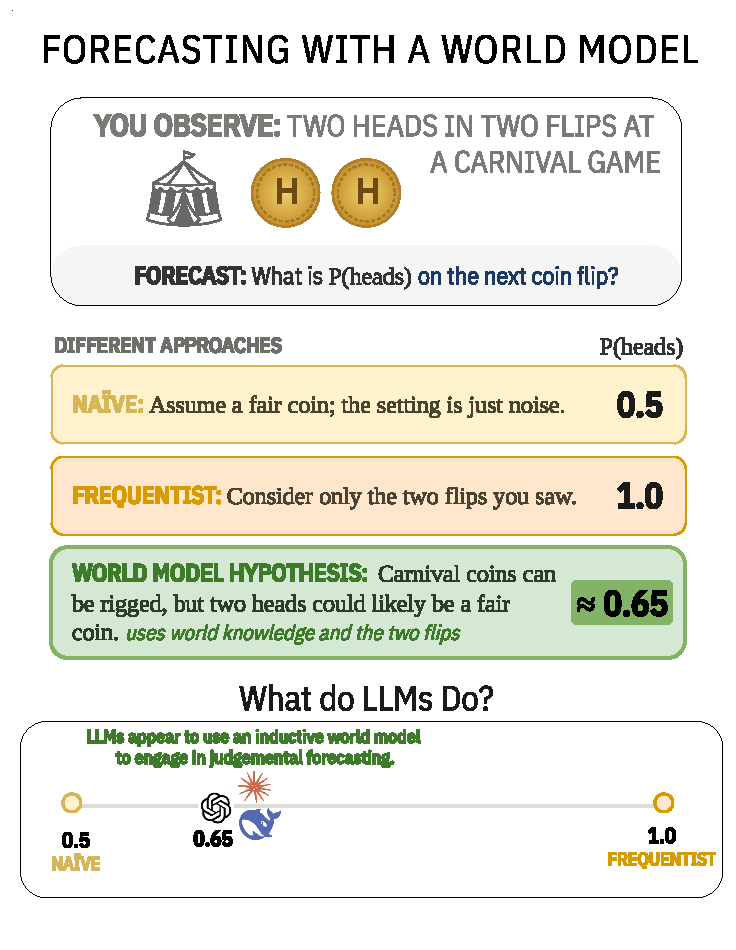
\includegraphics[width=353.04pt]{teaser_drawio_outlined.pdf}};
  \fill[white] (0,414) rectangle (353.04,456);

  % The scene adds the decision and payoffs within the existing footprint.
  \fill[white] (20,307) rectangle (333,412);
  \begin{scope}
    \clip[rounded corners=20pt] (24.5,309.5) rectangle (328.5,409.5);
    \fill[black!4] (24.5,309.5) rectangle (328.5,332);
  \end{scope}
  \draw[black,line width=.45pt,rounded corners=20pt]
    (24.5,309.5) rectangle (328.5,409.5);
  \node[text=teaserInk,font=\teaserfont\fontsize{13}{14}\selectfont]
    at (176.5,398) {PAY TO PLAY. TAILS WINS A PRIZE.};

  \node[text=teaserBlue,font=\teaserfont\fontsize{11.7}{12}\selectfont]
    at (91,378) {YOU};
  \node[text=teaserInk,font=\fontsize{12.2}{13}\selectfont]
    at (91,365) {Is it worth playing?};
  \node[text=teaserGray,font=\teaserfont\fontsize{11.7}{12}\selectfont]
    at (261,378) {OPERATOR};
  \node[text=teaserInk,font=\fontsize{12.2}{13}\selectfont]
    at (261,365) {Earns when you lose.};

  % Reuse the booth and coins from the original vector illustration.
  \begin{scope}[shift={(176.5,371)},scale=.82,transform shape]
    \clip (-19,-19) rectangle (19,19);
    \node[anchor=south west] at (-88.5,-365.5)
      {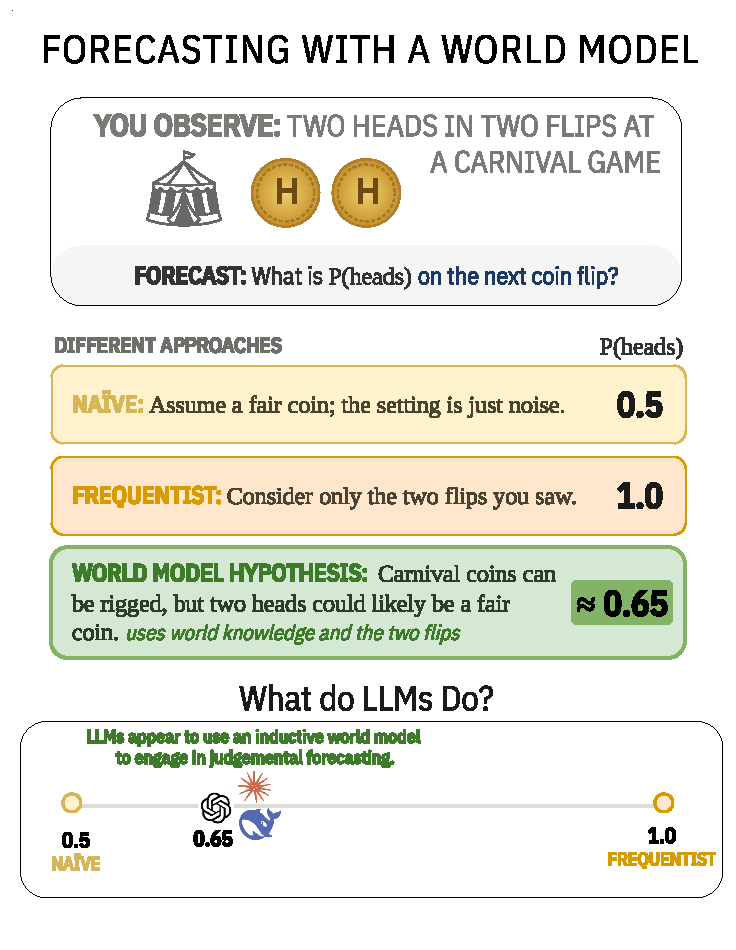
\includegraphics[width=353.04pt]{teaser_drawio_outlined.pdf}};
  \end{scope}
  \node[anchor=east,text=teaserGray,
    font=\teaserfont\fontsize{10.7}{11}\selectfont]
    at (173,346) {YOU OBSERVE:};
  \foreach \coinx in {190,212} {
    \begin{scope}[shift={(\coinx,346)},scale=.52,transform shape]
      \clip (0,0) circle (17.2);
      \node[anchor=south west] at (-137.25,-364.5)
        {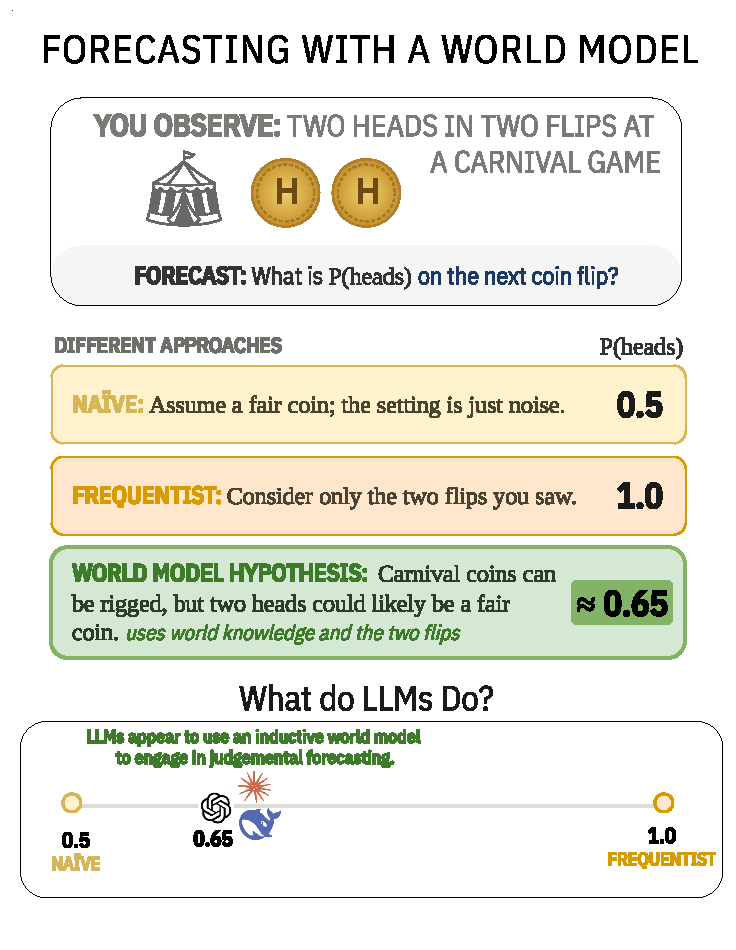
\includegraphics[width=353.04pt]{teaser_drawio_outlined.pdf}};
    \end{scope}
  }
  \node[text=teaserInk,font=\fontsize{12}{13}\selectfont]
    at (176.5,321)
    {{\teaserfont FORECAST:} What is P(heads) {\color{teaserBlue}on the next flip?}};

  \fill[teaserGreen,draw=teaserGreenDark,line width=1.4pt,rounded corners=8pt]
    (24.5,140.5) rectangle (330,194);
  \node[anchor=base west,text=black,
    font=\teaserfont\fontsize{11.7}{12}\selectfont]
    at (34.5,181.7) {WHAT THE LLMs SAID:};
  \node[anchor=base west,text=teaserInk,font=\fontsize{11.7}{12}\selectfont]
    at (34.5,168.5) {The carnival coin may favor heads.};
  \node[anchor=base west,text=teaserInk,font=\fontsize{11.7}{12}\selectfont]
    at (34.5,155.5) {Two flips alone are weak evidence.};
  \fill[teaserGreenDark,rounded corners=3pt] (275.5,156) rectangle (323,178);
  \node[font=\fontsize{16.5}{18}\selectfont] at (299.2,166.7)
    {$\approx$\,0.68};

  % The added game rules were not in the prompt that produced these means.
  \fill[white] (0,0) rectangle (353.04,139);
  \draw[gray!65,line width=.45pt,rounded corners=8pt]
    (24,77) rectangle (329,138);
  \begin{scope}[yshift=5pt]
  \draw[black!15,line width=1pt] (57,108) -- (296,108);
  \filldraw[fill=teaserYellow,draw=teaserGold,line width=.9pt]
    (57,108) circle (3.7);
  \filldraw[fill=teaserOrange,draw=teaserOrangeDark,line width=.9pt]
    (296,108) circle (3.7);
  % Positions encode the reported means .644, .681, and .712 on [.5, 1].
  % Logo copies use 8-bit alpha for compatibility with this XeTeX driver.
  \node at (125.832,109)
    {
\includegraphics[width=11.5pt]{teaser_openai.png}};
  \node at (143.518,115)
    {
\includegraphics[width=12pt]{../icons/claude.png}};
  \node at (158.336,106)
    {
\includegraphics[width=15pt]{teaser_deepseek.png}};
  \node[font=\teaserfont\fontsize{11}{12}\selectfont] at (57,94) {0.5};
  \node[font=\teaserfont\fontsize{11}{12}\selectfont] at (143.518,92) {0.68};
  \node[font=\teaserfont\fontsize{11}{12}\selectfont] at (296,94) {1.0};
  \node[text=teaserGold,font=\teaserfont\fontsize{10}{11}\selectfont]
    at (57,83) {NA\"IVE};
  \node[text=teaserOrangeDark,font=\teaserfont\fontsize{10}{11}\selectfont]
    at (286,83) {FREQUENTIST};
  \end{scope}
\end{scope}
\end{tikzpicture}
\null
\end{document}
